\documentclass[border=3pt,tikz]{standalone}
% Shared look for every TikZ figure in these notes.
% Included by each standalone figure file; also keeps the figures consistent
% with the colours used in the PDF and on the website.

\usepackage{tikz}
\usepackage{pgfplots}
\pgfplotsset{compat=1.18}
\usetikzlibrary{arrows.meta, decorations.markings, decorations.pathmorphing,
                patterns, calc, positioning}
\usepackage{amsmath}

% Series colours are the three validated categorical slots also used by the
% interactive widgets, so a path drawn in the printed notes and the same path on
% the website are the same colour. They clear the colour-vision-deficiency and
% contrast checks as a set; every path is direct-labelled as well, so colour is
% never the only thing carrying identity.
\definecolor{duPurple}{HTML}{68246D}
\definecolor{duBlue}{HTML}{2A78D6}
\definecolor{duRed}{HTML}{EB6834}
\definecolor{duGreen}{HTML}{1BAF7A}
\definecolor{duGrey}{HTML}{4D4D4D}

\tikzset{
  % heavier default lines and arrow tips, so diagrams stay clear when zoomed
  every picture/.append style = {line width=0.7pt, >={Stealth[length=3mm]}},
  axisline/.style   = {-{Stealth[length=3.4mm]}, line width=1.0pt, black},
  path1/.style      = {duBlue,   line width=1.6pt},
  path2/.style      = {duRed,    line width=1.6pt},
  path3/.style      = {duGreen,  line width=1.6pt},
  statedot/.style   = {circle, fill=black, inner sep=1.8pt},
  arrowhead/.style  = {decoration={markings,
                        mark=at position #1 with {\arrow{Stealth[length=3.4mm]}}},
                       postaction={decorate}},
  lbl/.style        = {font=\normalsize},
  slbl/.style       = {font=\small, duGrey},
  workfill/.style   = {duPurple, opacity=0.16},
}

% larger labels in plots as well
\pgfplotsset{every axis/.append style={label style={font=\normalsize}, tick label style={font=\small}, line width=0.9pt}}

% Entropy as microscopic disorder: particles confined to the left of a
% partition, then spread through the whole box once it is removed.
\begin{document}
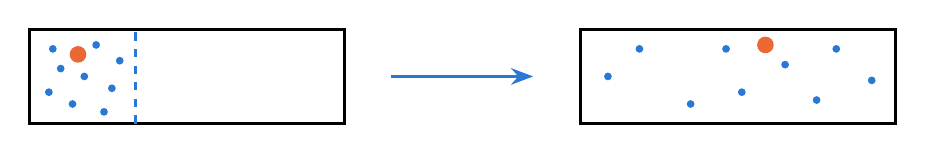
\begin{tikzpicture}[x=1cm,y=1cm]
  % before: particles left of the (dashed) partition
  \draw[line width=1.1pt] (0,0) rectangle (4.0,1.2);
  \draw[duBlue, dashed, line width=0.9pt] (1.35,0) -- (1.35,1.2);
  \foreach \x/\y in {0.3/0.95,0.85/1.0,0.25/0.4,0.55/0.25,1.05/0.45,1.15/0.8,
      0.4/0.7,0.95/0.15,0.7/0.6}
    \fill[duBlue] (\x,\y) circle (1.4pt);
  \fill[duRed] (0.62,0.88) circle (3pt);
  % arrow
  \draw[-{Stealth[length=2.8mm]}, line width=1.2pt, duBlue] (4.6,0.6) -- (6.4,0.6);
  % after: the same particles anywhere in the box
  \begin{scope}[shift={(7.0,0)}]
    \draw[line width=1.1pt] (0,0) rectangle (4.0,1.2);
    \foreach \x/\y in {0.35/0.6,0.75/0.95,1.4/0.25,1.85/0.95,2.05/0.4,2.6/0.75,
        3.0/0.3,3.25/0.95,3.7/0.55}
      \fill[duBlue] (\x,\y) circle (1.4pt);
    \fill[duRed] (2.35,1.0) circle (3pt);
  \end{scope}
\end{tikzpicture}
\end{document}
